%Feb 5, 2014
%Draft outline: MSIP
%Chris Carilli
\documentclass[preprint]{aastex}

\usepackage[top=1in, bottom=1in, left=1in, right=1in]{geometry}
\usepackage{amsmath}
\usepackage{graphicx}
\usepackage{mdwlist}
\usepackage{natbib}
\usepackage{natbibspacing}
\usepackage{caption}
\usepackage{subcaption}
\setlength{\bibspacing}{0pt}
\setlength{\parskip}{0pt}
\setlength{\parsep}{0pt}
\setlength{\headsep}{0pt}
\setlength{\topskip}{0pt}
\setlength{\topmargin}{0pt}
\setlength{\topsep}{0pt}
\setlength{\partopsep}{0pt}
\setlength{\footnotesep}{8pt}
\pagestyle{empty}
\citestyle{aa}

\newcommand{\compress}{\vspace{-0.12in}}


\def\kperp{k_{\bot}}
\def\kpar{k_{\|}}

\newcommand{\simgt}{\stackrel{>}{_{\sim}}}
\def\kperp{k_{\bot}}
\def\kpar{k_{\|}}
\def\k{{\bf k}}
\def\sky{{\theta}}
\def\HI{{H{\small I }}}
\def\HII{{H{\small II }}}
\def\xHI{{x_{\rm\HI}}}

%project description 20 pages total

\begin{document}

\title{Hydrogen Epoch of Reionization Array: Characterizing Cosmic Dawn}

\section{Overview} % 1 page ~ project summary? 
% Parsons, Carilli

% A statement of which of the four categories of MSIP is most appropriate
%for this proposal as the first sentence (see section II. Program Description).

%A. We propose HERA: next step in reionization roadmap
%B. Fulfill NWNH high-priority goals
%C. New understanding/techniques => faster, better, cheaper
%D. Brief summary of timeline: science along the way, major results before end-decade

{\it For the Mid-Scale Science Projects category of the Mid-Scale
Innovations Program}

The Hydrogen Epoch of Reionization Arrays (HERA) roadmap is a staged
program that uses the unique properties of the 21-cm line from neutral
hydrogen to probe the Epoch of Reionization and the preceding Dark
Ages.  During these epochs, roughly 0.3--1~Gyr after the Big Bang, the
first stars and black holes warm and reionize the neutral
intergalactic medium (IGM) that pervades the Universe following cosmic
recombination. Direct observation of the large scale structure of
reionization and its evolution with time, via the \HI 21-cm line, will
have a profound impact on our understanding of the birth of the first
galaxies and black holes, their influence on the intergalactic medium
(IGM), and cosmology.  CMB comparison statement? 

HERA was ranked the ``{\it top priority in the Radio, Millimeter, and
Sub-millimeter category of recommended new facilities for mid-scale
funding}" as part of the {\it New Worlds, New Horizons of Astronomy
and Astrophysics} decadal survey (\citealt{astro2010}; hereafter
NWNH).  The HERA roadmap initially envisioned a series of radio
interferometers constructed throughout the decade, starting with the
existing Donald C. Backer Precision Array to Probe the Epoch of
Reionization (PAPER) and the Murchison Widefield Array (MWA)
instruments aimed at characterizing foregrounds and laying the
groundwork for a statistical detection of the HI 21cm signal through
the power spectrum.  A second-generation HERA instrument would measure
the evolution of the power spectrum in detail and reveal how early
structure in the Universe formed. A third-generation instrument would
image the typical structures during reionization.

While receiving only a fraction of the funding for HERA phase I
recommended in NWNH, the MWA and PAPER projects have made
major strides in understanding the techniques required to disentangle
the reionization signal from the strong radio continuum foreground
confusion. Based on this new understanding of array response to the
celestial signal, we are ready to build the next generation of HERA in
stages of 127 and 331 elements, observing in the 50--225-MHz band.
These stages increase the sensitivity by two orders of
magnitude over to the current arrays, through the use of an
optimal configuration of 14m diameter receptor elements, and a
tailored analysis technique that mitigates foreground contamination.
The proposed experiment delivers HERA-II science at a cost
substantially below originally envision in NWNH:

% might remove 1st phrase in 1st sentence in para above

\vspace{-4pt}
\begin{itemize}\setlength{\parskip}{0pt}\itemsep0pt

\item HERA~127 will measure the rise and fall of the EoR power
spectrum, constraining the timing and duration of reionization.

\item HERA~331 will measure EoR fluctuations over a variety of spatial
scales to determine the features and distribution of the first objects
that dominate cosmic reionization. HERA~331 will also extend precision
power-spectrum observations into the Dark Ages, and directly image the
largest scale structures in the IGM during reionization.

\end{itemize}
\vspace{-4pt}

The proposed program produces a sequence of dedicated experiments
optimized to fulfill the NWNH goal of characterizing the evolution of
the HI 21cm power spectrum during cosmic reionization. In
its final stages, HERA will be capable of imaging the neutral
IGM --- a task previously only considered for third-generation
instruments. This proposal includes funding for both the
telescope development and construction, as well as for the key
scientific data analyses for each stage of the project.

\section{Science} total = 8 pages

\subsection{Introduction}    % 1 page + 1 fig = simulated Tb cube + PS evolution
% Furlanetto, Carilli

%i.physical concepts: reionization and dark ages
%ii. Current knowledge: various constrai	nts, 1st galaxy studies...
%iii. Important role of 21cm studies highlighted in NWNH
%a. Typical ideal sim results: T_B vs. z 'cube' and corresponding power spectrum evolution (Fig)
%b. introduce some of the important parameters/processes explored: when? how? bubble scale? sources? inside out? [much of this could be left for below?)
%c. reemphasize that current knowledge is nil, yet demand is high
%d. emphasize unique (only?) probe of dark ages

The period beginning with the the birth of the first stars, and culminating with the full
ionization of the intergalactic medium (IGM) some 500 Myrs later, 
represents one of the last unexplored phases of cosmic evolution. During the Dark Ages
($z\simgt15$) and the Epoch of Reionization ($z\sim$15--6), a wealth
of astrophysical and cosmological phenomena are at work. The precise
properties of the IGM depend on the cosmic density field, the nature
and distribution of the first luminous sources (eg. typical masses, UV
escape fractions, biased structure formation), the efficiency and
abundance of heating sources (eg. X-ray binaries, shocks, or even dark
matter annihilations), the formation of the first supermassive black
holes, and the relative velocity of baryonic matter and dark-matter
halos, among other effects.  Exploring these early structures and
their effects on each other and their environments was one of the top
three ``{\it priority science objectives chosen by the [NWNH] survey
committee for the decade 2012-2021.}"

To date, a number of indirect probes have been used to understand
cosmic reionization. These include observations of resonant scattering
of Ly$\alpha$ by the neutral IGM toward distant quasars (the
'Gunn-Peterson' effect) \citep{fan_et_al2006}, kinetic
Sunyaev-Zel'dovich anisotropies in the CMB temperature
\citep{zahn_et_al2012_trunc}, the CMB \citep{planck_et_al2013} and its
polarization \citep{page_et_al2007}, and the demographics of
Ly$\alpha$ emitting galaxies \citep{treu_et_al2013}, as summarized in
the left-hand panel of Figure~\ref{fig:x_i_Xray}. The latest analysis
of these constraints suggests that the IGM may have been substantially
neutral even at $z \sim 7$ to 8 (as high as $F_{HI} \sim 0.5$), with
a tail of finite ionization ($\sim 0.1$) extending to high redshift
($z \sim 15$), driven by very early galaxy formation (Robertson et
al. 2013).  Unfortunately, these important results have limited
reach: the Gunn-Peterson effect and related phenomena saturate at low
neutral fractions, and the CMB provides only an integral measure of
the Thomson optical depth of the IGM back to recombination. Moreover,
many of these indirect observations are in tension with one another,
underscoring both the difficulty in their interpretation and the
complexity of the reionization process.

The 21-cm emission line from neutal Hydrogen has been recognized as
potentially the most powerful probe of cosmic reionization and 
the dark ages \citep{morales_wyithe2010,
furlanetto_et_al2006}, as emphasized in NWNH: ``{\it The panel
concluded that to explore the discovery area of the epoch of
reionization, it is most important to develop new capabilities to
observe redshifted 21-cm \HI emission, building on the legacy of
current projects and increasing sensitivity and spatial resolution to
characterize the topology of the gas at reionization.}"  The HI 21cm
line provides a direct method to image the evolution of the primordial
IGM, opening a unique window into the complex astrophysical
interplay between the first luminous structures and their
surroundings. Given that the signal is a spectral line, the HI 21cm
studies result in a full three-dimensional view of the evolution of
large scale structure during this 'last frontier' in observational
cosmology. The direct observation of the primordial IGM via
the HI 21cm line would be an achievement comparable in importance to
the detection of anisotropies in the CMB.

In the past decades, considerable effort has gone into modeling the
complex astrophysics of reionization
(e.g. \citealt{shapiro_giroux1987, haiman_loeb1997,
furlanetto_et_al2004, santos_et_al2010}). Figure ?? shows a simulation
of the expected evolution of the HI 21cm signal during
reionization. The HI 21cm fluctuations initially rise above those
expected from the Cosmic density field due to the growth of ionized
bubbles on a characteristic scale of a few to 10arcmin. This scale is
set by the clustering of early galaxy formation, as well as by
propagation effects through the IGM. The signal then declines as the
IGM becomes fully ionized.  The typical surface brightness for the HI
21cm emission is a few to 10 mK.  Imaging the evolution of these
typical structures requires the full collecting area of the
SKA. However, precusor experiments, such as PAPER and the MWA, are
underway which are designed to make the first statistical discovery of
this signal through power spectral and related analyses.

We emphasize that basic constraints on theoretical models are still
rudimentary, and the most fundamental questions concerning the process
of reionization remain open.  When did reionization occur, and over
what timescale?  What objects dominated the radiation field?  How were
the objects distributed?  What were the most important feedback
mechanisms in the transition from the first stars to first galaxies,
and how did they affect these populations?  {\it HERA provides the key
measurements that are needed to advance our understanding of early
galaxy formation and cosmic reionization.}

Figures: F(HI) vs z;  HI Tb cube + PS evolution


\subsection{HI reionization and dark ages science} % 4 pages total examples using hera 331, plus a number of figures

i. F(HI) vs. z: HERA vs. other techniques (Fig) -- emphasize constaints in unexplored territory
% Bowman


\subsubsection{Detecting and characterizing the power spectrum}
\emph{ii. PS sensitivity at fixed z: 127, 331 (Fig)}
% Pober, Dillon
\begin{figure}[t]\centering
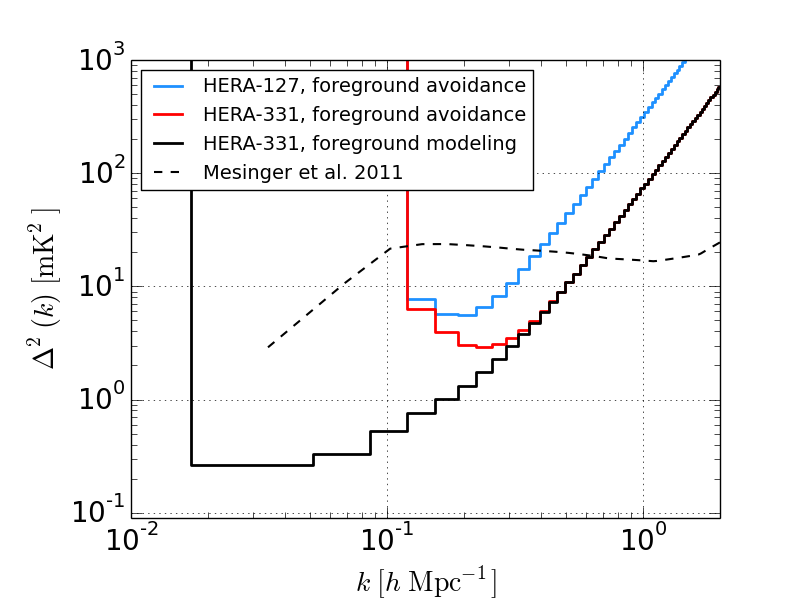
\includegraphics[width=\textwidth]{plots/Pspec/eor_pspec_2014.png}
\caption{Power-spectrum sensitivities for three stages of
HERA (solid) relative to a fiducial ionization model (dotted line; $\xHI=0.37$, $z=9.0$).  
Sensitivity curves reflect a staged array size and
a staged improvement in analysis software that expands the range
of modes falling into the EoR Window \label{fig:PspecSensitivity}}
\end{figure}

A season of observing with HERA-127 will yield high-significance constraints on the 21 cm power spectrum across a wide range of k modes and redshifts.  In Figure we show the $z=9$ power spectrum predicted by the publicly available 21cmFAST software \citep{mesinger_et_al2011}, along with $2\sigma$ HERA sensitivities.  Using the conservative delay-spectrum approach employed in Parsons et al. 2014, we find that HERA-127 can achieve a $> 10\sigma$ detection of fiducial power spectra over a broad range of redshifts.  The subsequent observing season with HERA-331 can increase this detection significance to over $25\sigma$ using the same methods.  With detailed foreground modeling, a more sophisticated power spectrum estimator could increase the size of the ``EoR window", the region of Fourier space with minimal foreground contamination. This would allow for an overall detection significance of up to $90\sigma$, along with access to lower $k$ modes and therefore qualitatively different physics.  Such a high sensitivity measurement would also allow one to go beyond constraining parameters, testing rather than assuming the underlying theoretical framework.

\subsubsection{Astrophysical parameters from the power spectrum}
\emph{iii. Various covariance analyses: constraints on different physical processes (Liu/Pober analysis). but
please -- keep this down to a couple of incisive figures and fiducial models. wall paper doesn't sell very well. }
% Liu, Pober, Dillon
The power spectrum measurements with HERA-331 are sensitive enough to place constraints on theoretical models that describe the reionization process.  To first order, the major features of the power spectrum (as simulated by 21cmFAST) can be parameterized by three terms: $\zeta$, the efficiency at which galaxies release ionizing photons into the IGM; $T_{\rm vir}$, the minimum virial temperature of halos that produce ionizing photons (a proxy for the minimum mass of the galaxies that drive reionization); and $R_{\rm mfp}$, the mean free path for ionizing photons traveling through the IGM, which is determined the prevalence of dense Lyman limit systems.  Current observations limit the value of these parameters to within an order-of-magnitude (or worse, in the case of $T_{\rm vir}$).  Figure \ref{fig:ErrorEllipses} shows the constraints on each of these parameters achievable with multi-redshift HERA-331 power spectrum observations.  We expect to constrain these parameters to better than 5\% with a conservative approach to foregrounds , and even better with explicit foreground modeling \citep{pober_et_al2014}.

\begin{figure*}[t]\centering
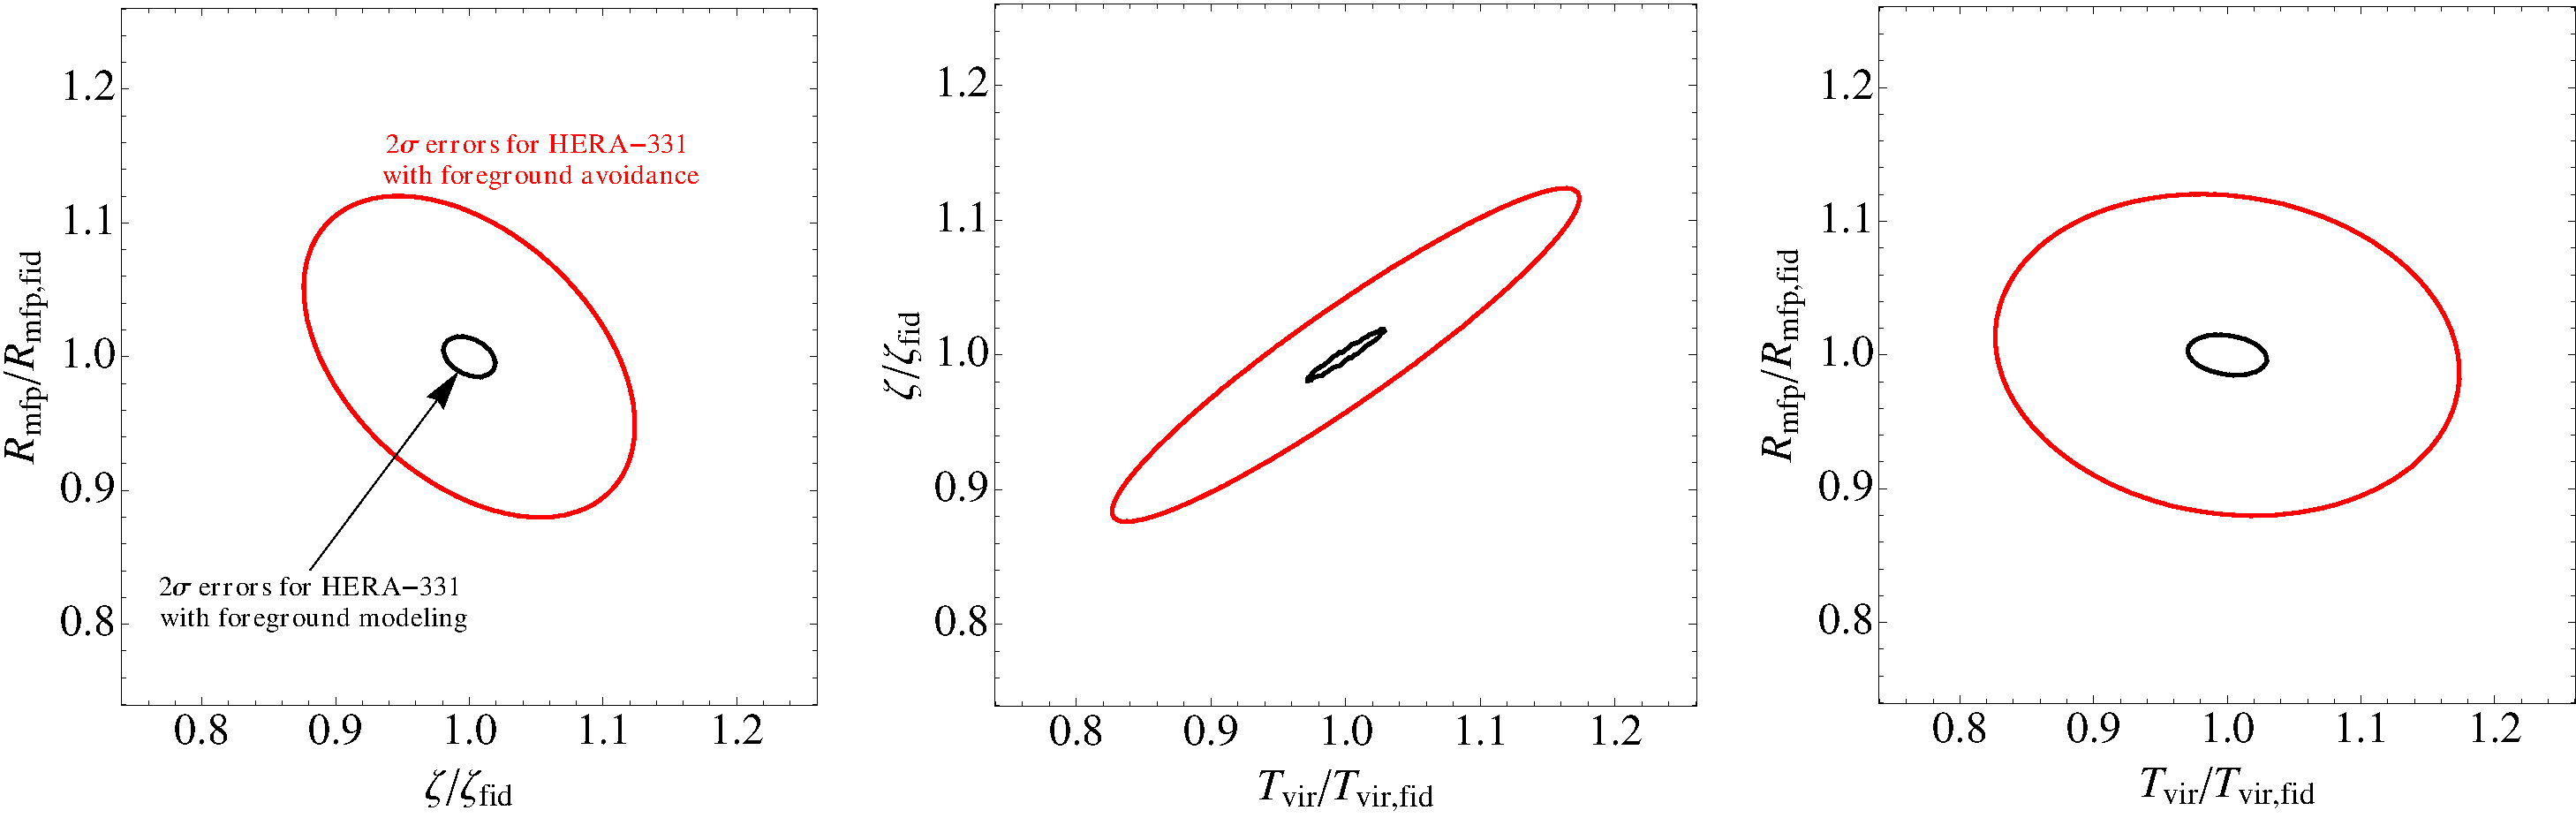
\includegraphics[width=\textwidth]{plots/Pspec/OPTMIDellipses.pdf}
\caption{Pairwise $2\sigma$ error ellipses for $T_{\rm vir}$, $\zeta$, and $R_\textrm{mfp}$, in each case divided by their fiducial values.  HERA-331 projections using existing foreground avoidance techniques are shown in red, while projections using more advanced foreground modeling techniques are shown in black.  The former represent $\sim 5\%$ constraints, while the latter represent $\sim 1\%$ constraints.\label{fig:ErrorEllipses}}
\end{figure*}


% Jacobs
\subsubsection{Imaging HI}
iv. Imaging large scale structure: simulation (Fig) 
With a nearly completely sampled aperture over 300m across, HERA will have the collecting area of Arecibo but with 500x the survey speed it presents the opportunity for directly imaging reionization.  After 100 hours on a single field (achievable in 200 nights, or just over one season) HERA will reach a surface brightness sensitivity of 50 $\mu$Jy compared with typical brightness temperatures of EoR models which often peak above 400 $\mu$Jy.

In imaging, as in the measurement of the power spectrum, noise and foreground residual are comparable limiting factors. Using the foreground filtration methods developed for power spectrum estimation, we can remove foregrounds exactly as done for the power spectrum estimation --filter the ``wedge'' in power spectrum space-- before imaging.  This ``foreground avoidance'' scheme effectively limits the bandwidth (line of sight modes) over which the residuals can be imaged without signal loss.  In Figure \ref{fig:imaging} we demonstrate the sensitivity of imaging in this mode assuming a conservative 1MHz of effective bandwidth, 12Mpc along the line of sight.  The brightest structures in the redshift 8 input simulation are detectable at the SNR$>10$ level.

\begin{figure}[t]\centering
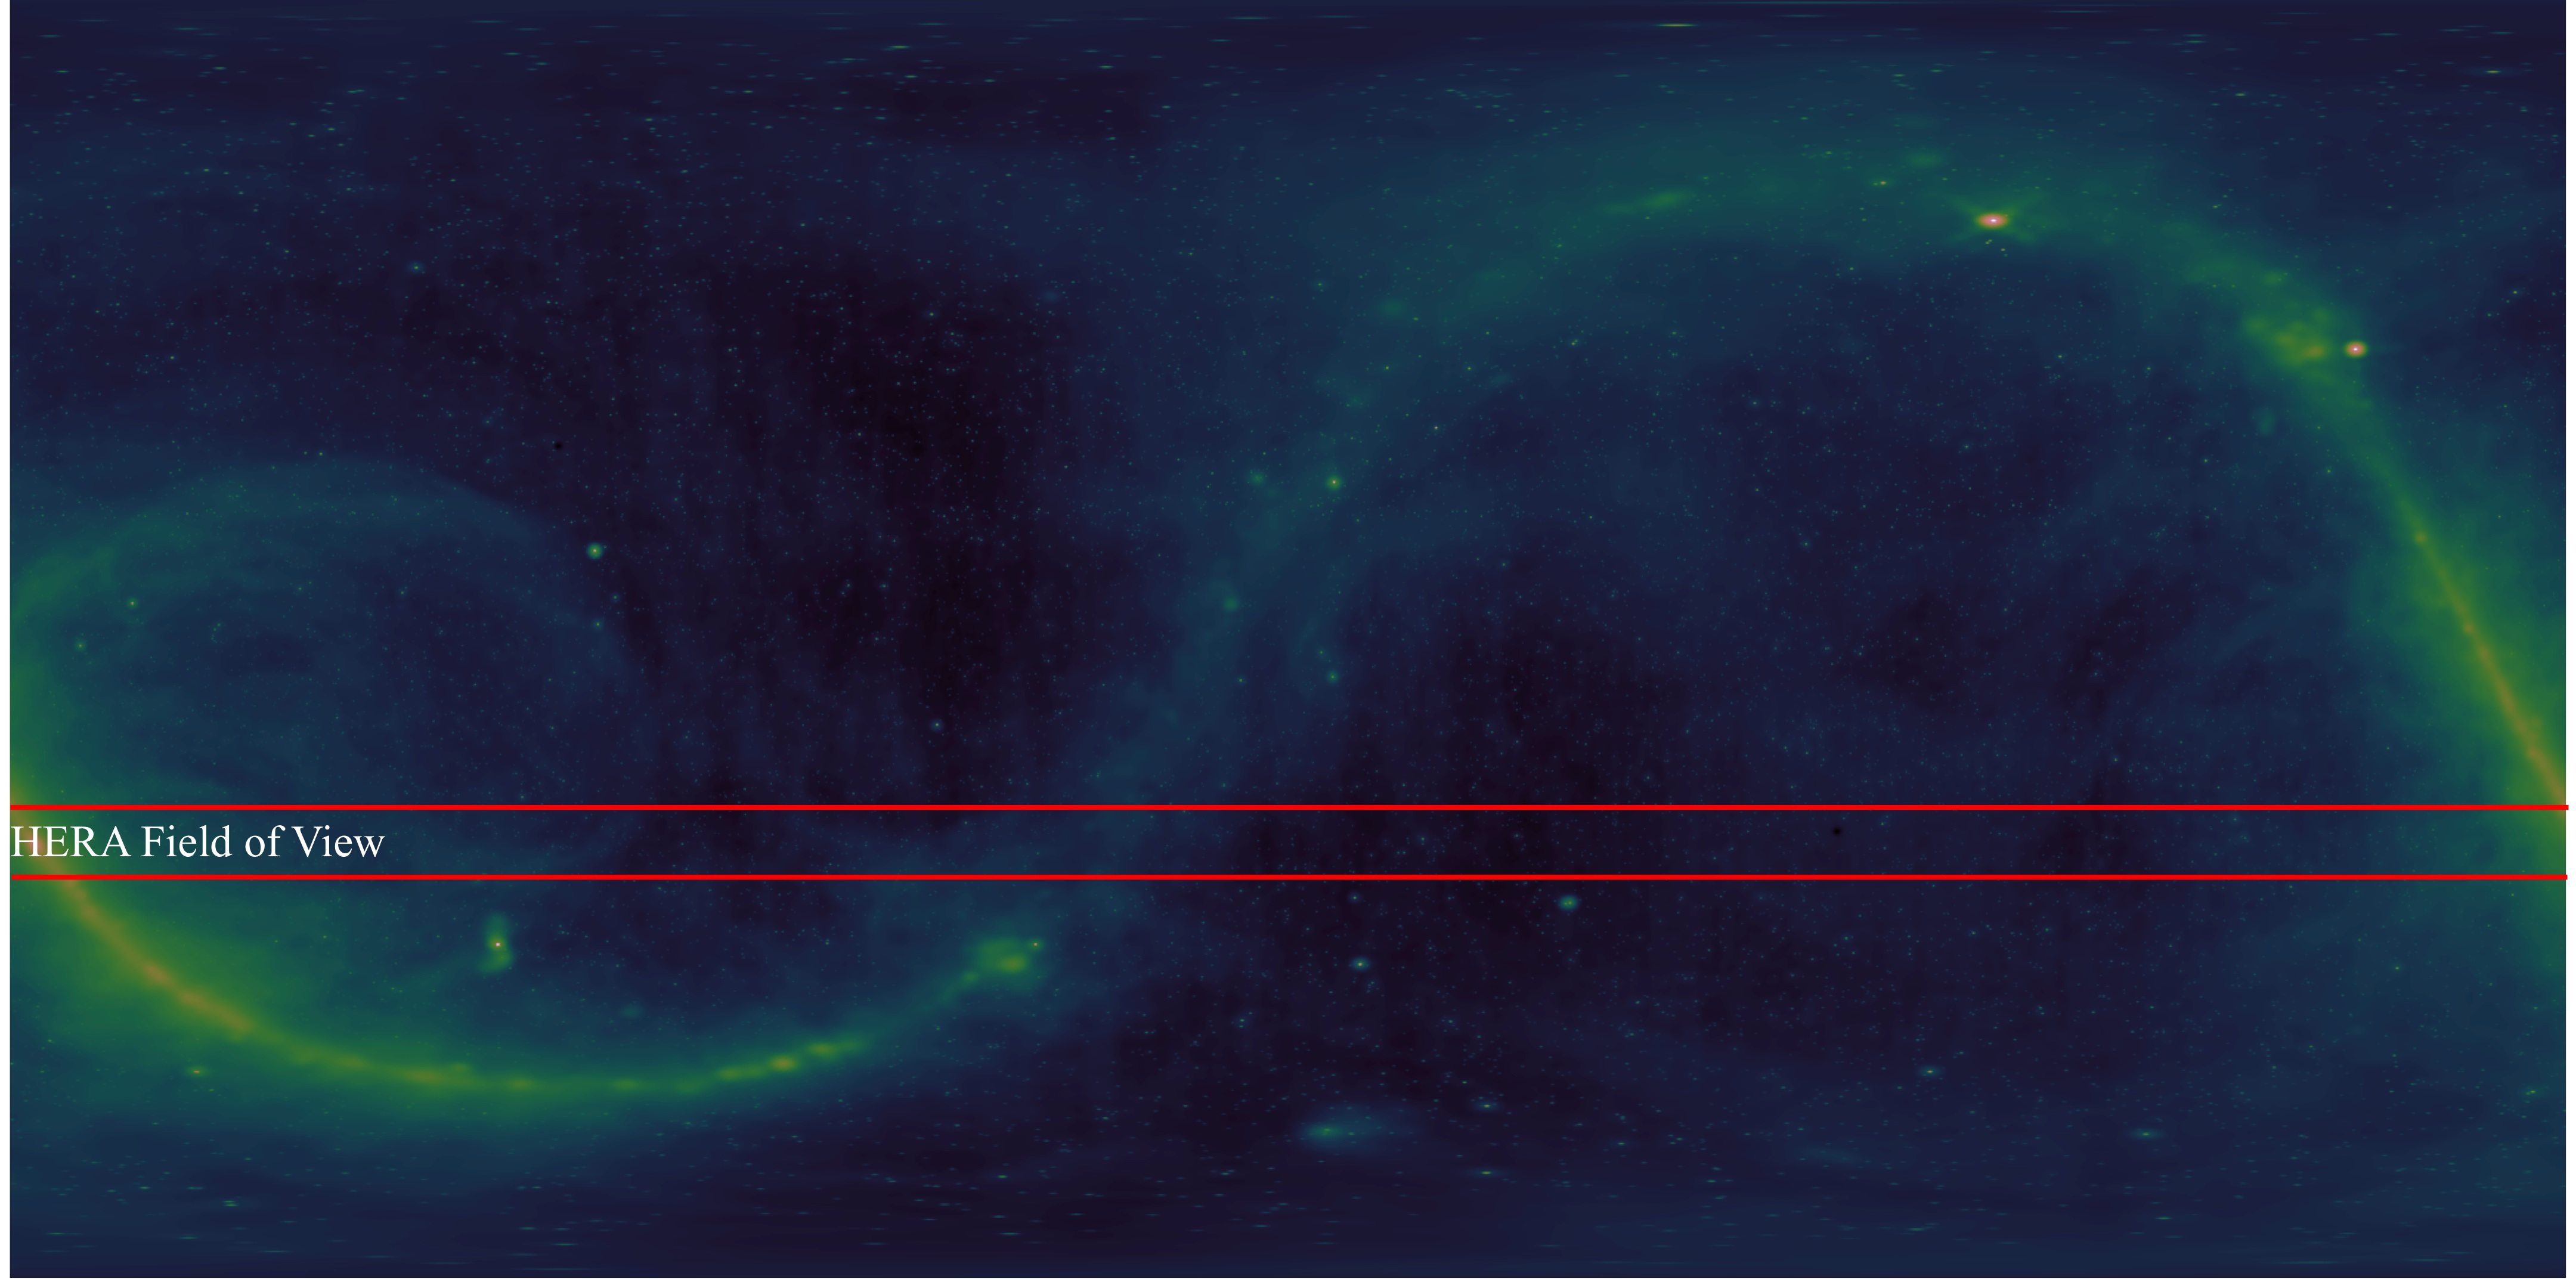
\includegraphics[width=\textwidth]{plots/Imaging/HERA_FoV.jpg}
\caption{The HERA stripe.  At 150MHz ($z=8.5$) the HERA field of view is 8\arcdeg.  With a nearly completely sampled aperture over 300m across, HERA will have the collecting area of Arecibo but with 500x the survey speed. Each night it will drift scan 2600 square degrees for a survey volume of 50 $Gpc^3$.  The stripe includes the GOODs south field, one of the best studied regions of sky. \label{fig:HERA_FoV}}
\end{figure}

With a resolution of 60Mpc and survey volume of 1Gpc in a single field of view HERA images will probe structure on scales well beyond any deep, high redshift field contemplated. For comparison, note that the entire Great Observatories Origins Deep Survey (GOODS), where 40\% of all objects at $z > 6$ have been found, is only (30Mpc ) 15\arcmin  across. Using deep HERA images it will be possible to make targeted observations of early galaxies known to be in the center of large scale bubbles, directly observe clouds responsible for Ly$\alpha$ absorption, and correlate large scale intensity surveys.


 
\begin{figure}[t]\centering
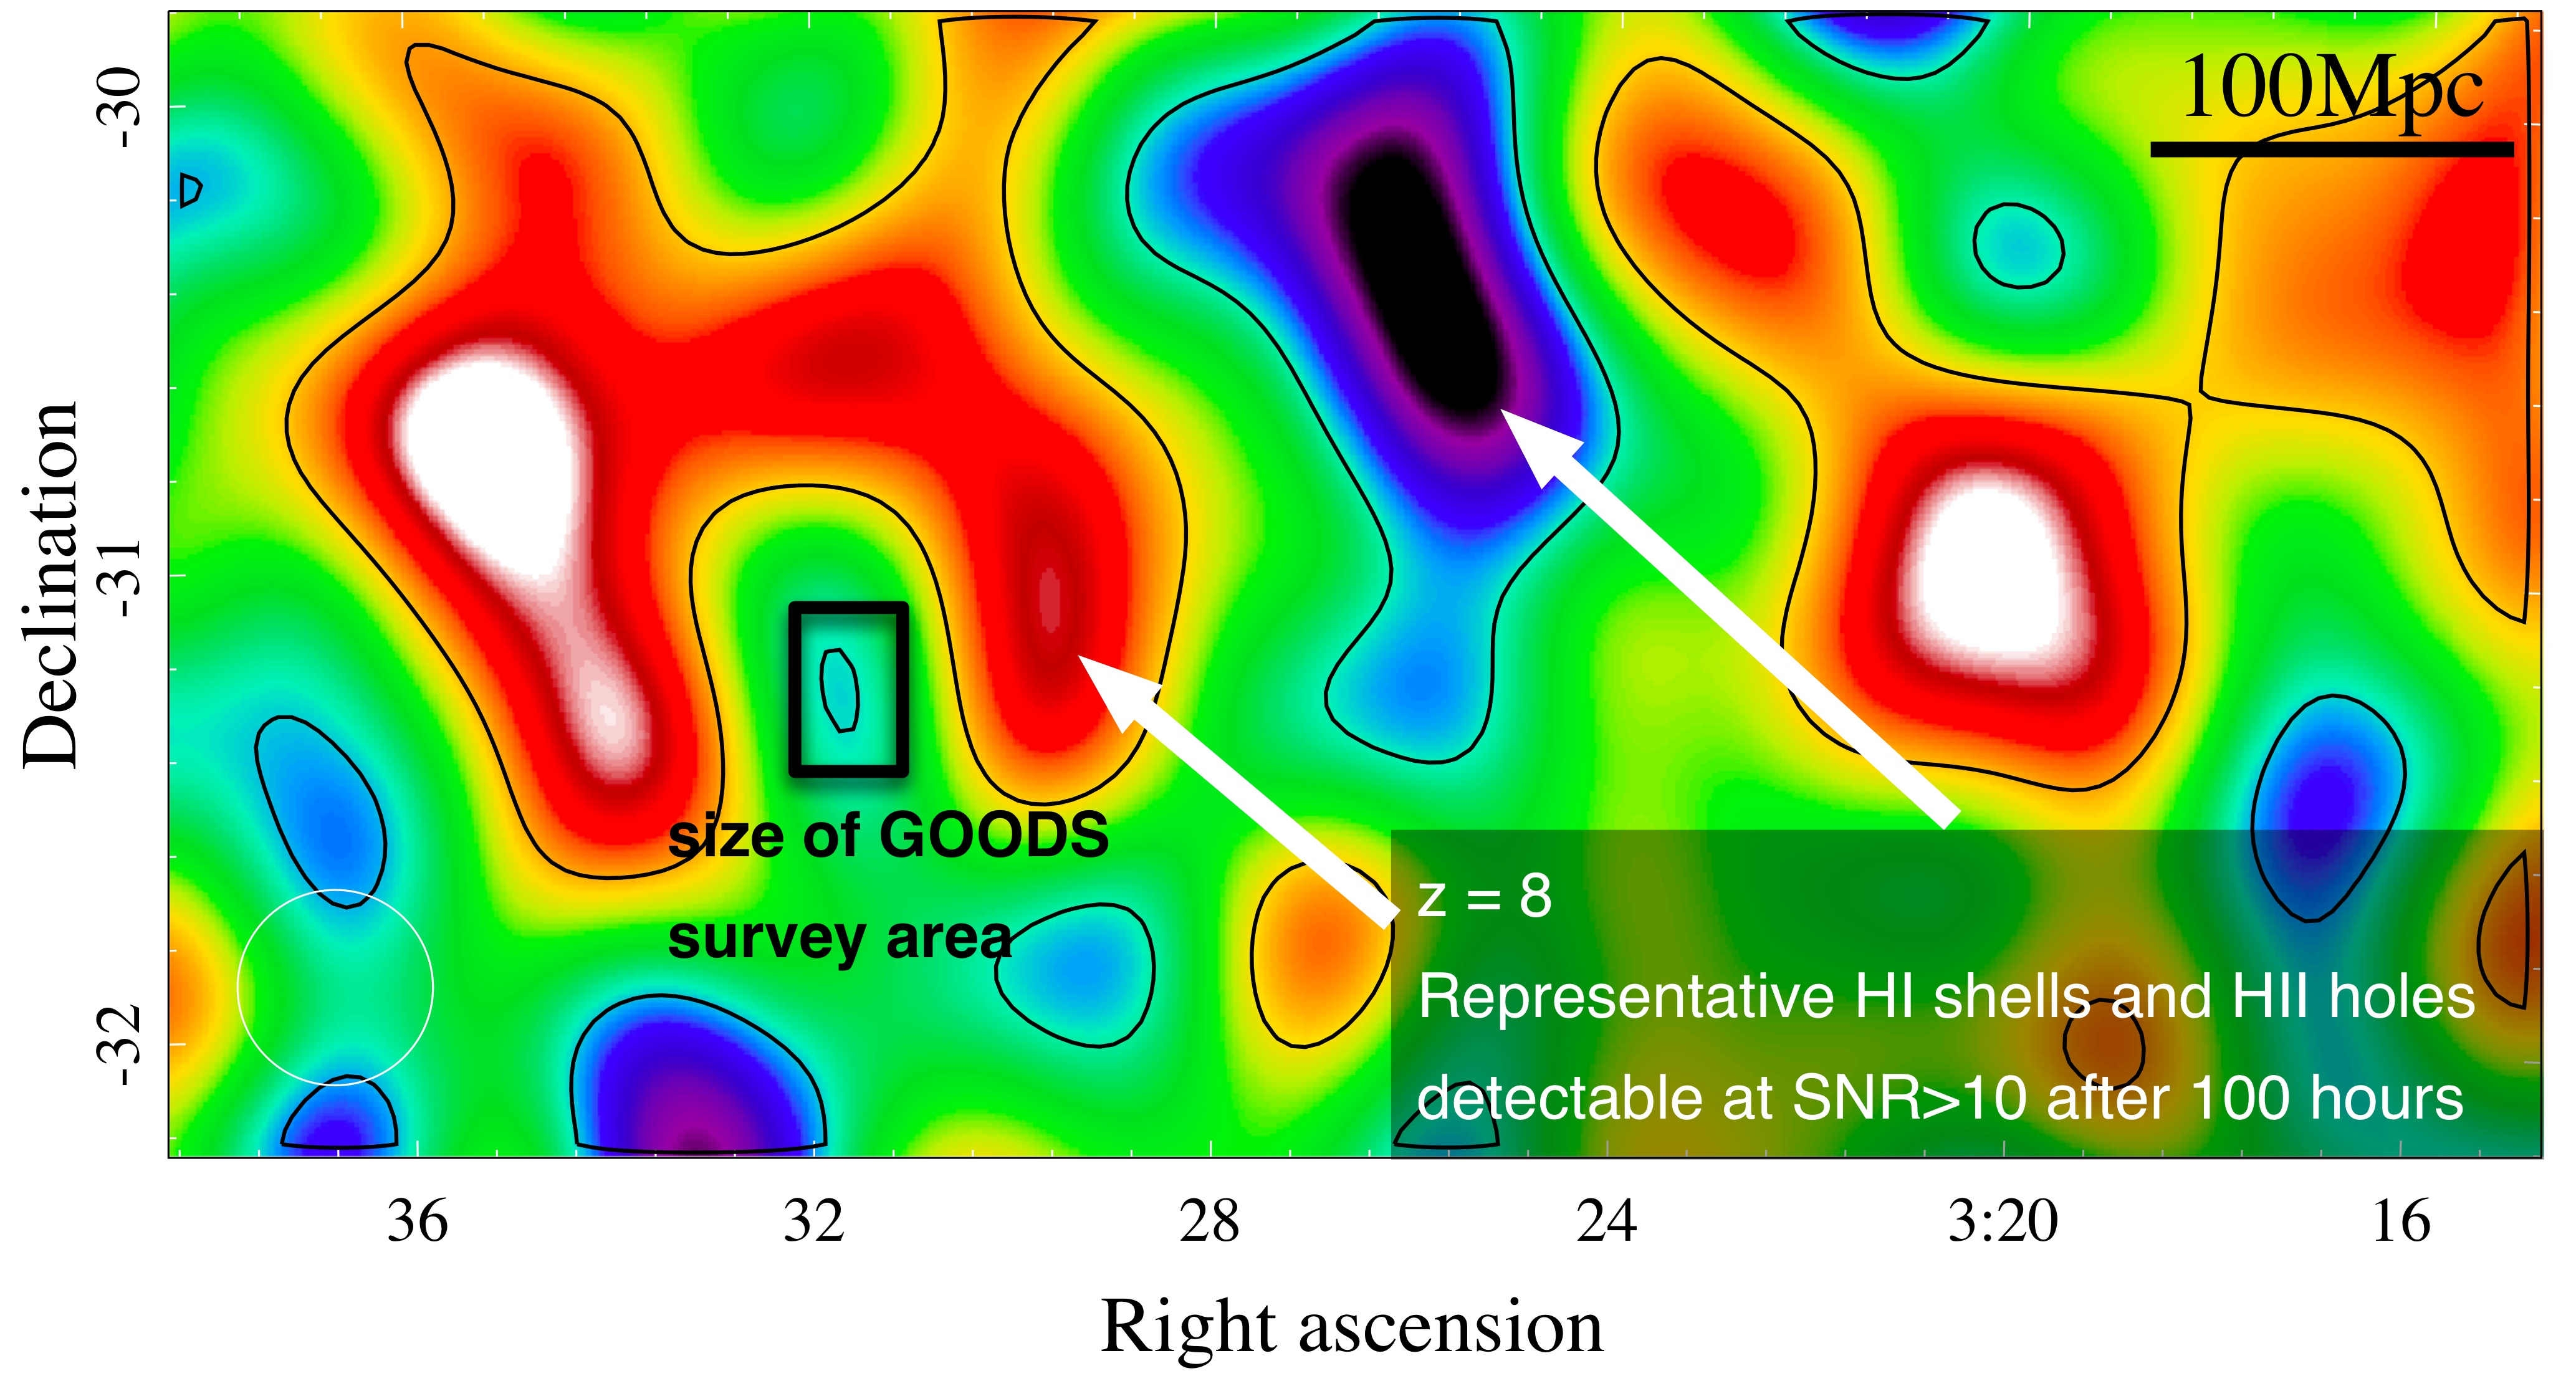
\includegraphics[width=\textwidth]{plots/Imaging/HERA_331_z8_SNR_annotated.jpg}
\caption{\small
With sensitivity highly concentrated at the largest scales, HERA is capable of directly imaging HI during reionization.  Shown here is a simulation of EoR emission (McQuinn 2009) as imaged by HERA with noise equivalent to 100 hours of observation and bandwidth equivalent to the moderate foreground model. %XXX are we using the language of pober et al? 
Contours enclose regions with signal to noise above 10.  The regions detected on scales of $\sim$100 Mpc are bracket the size scales probed by deep galaxy surveys (cf. the GOODs-South survey volume where 40\% of all galaxies above redshift 7 have been detected.)  The GOODs field itself is located within the HERA stripe, just 3 degrees outside of the image shown here.
\label{fig:imaging}}
\end{figure}    

\subsubsection{Imaging as a probe of non-gaussianity}
\emph{a) Imaging as a probe of non-Gaussianity and topology of reionization (Fig from Watkinson \& Pritchard)
[Not sure if this belongs here, should discuss: b) Bayesian imaging (Figs from Paul Sutter).  
Perhaps a broader impact on the radio community too?]}
% Morales, Tegmark

\subsubsection{Early IGM heating}
\emph{v. Approaching Dark ages (z=20 to 30): early Xray heating? other (Fig - Liu models)}
% Liu, Dillon, Hewitt
\begin{figure}[t]\centering
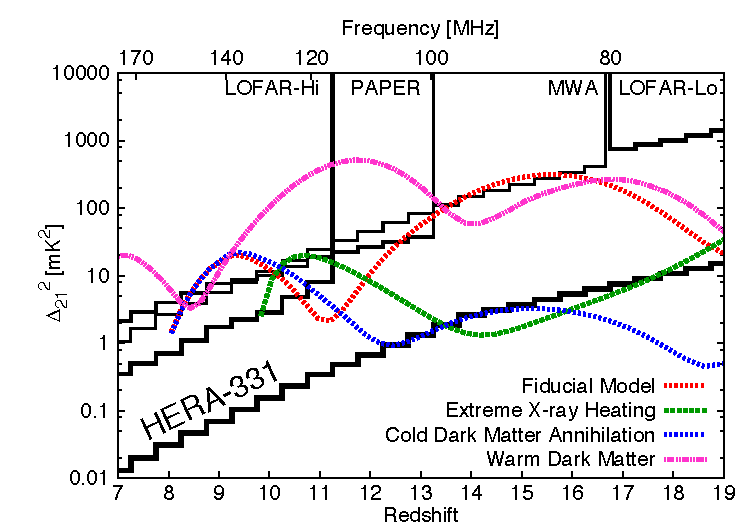
\includegraphics{plots/Xray/HERA_II_compare_kp1_whoriz_20pt.pdf} 
\caption{\small 
At low frequencies, HERA opens a window to
pre-reionization physics at the end of the Dark Ages. Plotted are power spectrum amplitudes (at $k =
0.15h$~Mpc$^{-1}$) for various IGM heating models \citep{mesinger_et_al2013},
with predicted HERA sensitivities.
}\label{fig:Xray} \end{figure}

With high thermal noise sensitivity throughout the observing band, HERA represents an opportunity to push the redshift frontier of current-generation instruments, extending observations to the pre-reionization era in an uninterrupted way.  Doing so will allow a measurement of an earlier peak in the $21\,\textrm{cm}$ power spectrum, corresponding to an era of IGM heating from various X-ray sources.  Theoretical expectations span a wide range of possible scenarios for IGM heating, and Figure \ref{fig:Xray} shows several that were examined in \cite{mesinger_et_al2013}, with HERA's sensitivity overlaid.  It is clear that HERA possesses the sensitivity to easily detect and distinguish between these possibilities, placing the first observational constraints on the pre-reionization epoch, including possible bounds on exotic physics such as dark matter annihilation.


vi. 21cm forest: perhaps a paragraph on possibilities of small scale structure, if we can find radio galaxy? (Fig) 
% Carilli, Furlanetto -- Forget it.  Too much explanation needed. 

vii. Cross-correlation science: perhaps montage Fig showing HI(Tb), galaxies, dark matter... at given epoch
\cite{lidz11}
% Aguirre, Tegmark

a. Provide environmental context for ALMA/JWST 1st galaxy studies

b. CMB pol 

c. CO/CII IM: optimistic or wrong timescale?
  
d. note: xcorr further mitigates continuum systematics

e. Anscillary science with PAPER 128: transients, solar 
% de Boer

\subsection{Where we are right now: PAPER, MWA}  % 2 pages

i. describe arrays, state design driven by new understandings as delineated below (Fig)
% Parsons, Bowman

ii. Using new techniqes, current best limits  (Fig)
% Parsons, Morales

iii. what will happen in next 2 years: hopefully detection, but no more

%iv. LOFAR/MWA/PAPER 
% Carilli
Three reionization path-finder array experiments are currently
operational: LOFAR, MWA and PAPER. All three are designed to have the
sensitivity to make the first statistical detection of the neutral
IGM. However, the HI line experiment is very challenging due to
foreground continuum emission some four orders of magnitude brighter
than the expected line signal.  The three experiments offer very
significant complementarity, with different intrinsic systematics and
different approaches to foreground mitigation. We emphasize that, for
such an important discovery, multiple approaches are critical in order
to check and verify any claimed (likely low S/N) detection amidst the
substantial systematic uncertainties. The first detection of
the neutral IGM is not the end of reionization studies, just the 
beginning. Recall that some four decades separated the first detection
of the CMB from the first statistical characterization. 


iv. HERA II: 'gauranteed' detection, full characterization, dark ages, imaging
% Aguirre

v. Move 'analysis' stuff here?


\section{Challenges} % 2 pages

\subsection{Foregrounds}  % 1.5pages
% Parsons, Morales

i. relative intensities (Fig: Continuum from MWA)

ii. Details on Delay Spectrum approach

a. key: 3D k-space: show wedge and discuss. chromatic sidelobes with characteristic freq scale 
set by baseline length

b. analysis focuses on line-of-sight PS dimension

c. work in EoR window.  different window levels, depending on effective horizon

d. drives design to redundant array: helps calibration, add spectra coherently

e. dictates geometry of antenna elements and other RF stuff. avoid standing waves of given length. 

f. area: drives sensitivity as used in section 2

g. some words about why compact, hex array 

\subsection{Other Challenges} % 0.5 pages

i. Interference: Karoo RFI plots  FIG 
% Jacobs

i. Polarization 
% Moore, Aguirre

D. Ionosphere: 

i. short baselines and narrowish FoV

ii. direction dependent gains?


\section{HERA design and project} % 8 pages

\subsection{Lessons learned recap} % 0.5 page
% Parsons, Morales

reemphasize design dictated by new understanding

\subsection{Project component details}  % 6 pages
% DeBoer to parse
In terms of hardware, HERA is a simple and straightforward system.  The element
itself is a fixed zenith-pointing 14-meter segmented prime-focus paraboloid with a high screen
to minimize cross-talk between elements (which are spaced 14.3 meters on a
hexagonal grid.  Figure \ref{fig:configuration} shows the layout of the array.  The $f/D$ of
the paraboloid is 0.32, so that the focal length, $f$, is less than 5 meters to meet the 
standing wave specification at the delays of interest of more than 60 dB of attenuation at delays 
greater than 15 ns.

The active feed sends back the entire dual-polarization analog bandwidth on standard
coaxial cable to an aggregation point called a ``node'', which services 
about 15 antennas.  This cable length is kept short to keep any standing
wave contamination outside of the delay-space of interest for power spectrum
measurements.  The node amplifies, filters, digitizes and transmits the signal data stream
back to a central location 

i. compact hex grid array
% de Boer

ii. 14m elements + broad band (active) dipole feed
% de Boer, Bradley

iii. Signal transport: RF to nodes, digitize at nodes. fiber to correlator. 
% Wirtheimer?

iv. Digital stuff: emphasize 'solved problem'. Casper work. block diagrams...
% Parsons

C. Post correlator data path
% Aguirre, Moore

i. local storage

ii. transport to data centers

iii. data centers: access? 

D. Data analysis [Move up?]

i. Calibration 
% Aguirre, Morales

ii. Continuum and removal
% Morales

iii. Delay spectrum analysis
% Pober

iv. Other (related) approaches: Bayes, z-variance,
% Liu, Carilli

v. HI imaging
% Jacobs

E. Array monitoring/maintenance: daily, weekly health monitoring
% de Boer

F. Aspirations [move to facilities section?]

i. FFT correlator

ii. other

\subsection{Five year Schedule and deliverables} % 0.5 page
% De Boer

i. stages and science

ii. first science within 3 or 4 years

iii. main science results before end of decade


\section{Broader impacts} % 1 page
% Aguirre

A. pre and post-doctoral students

B. South Africa connection

i. professional development/exchanges

ii. broader outreach in SA

C. Broader astronomy community

i. Data access: transients, SETI, ionosphere

ii. Cross correlation: CMBpol, CO/CII IM

D. Casper open source: good example to build from


\section{VI. Summary: why us and why now?} % 0.5 pages
% Parsons

that's obvious


\clearpage
\setcounter{page}{1}
\thispagestyle{empty}
%\bibliographystyle{apj}
%\bibliographystyle{hapj}
\bibliographystyle{jponew}
\bibliography{biblio}

\end{document}

